% A single module with data flow for forward/backward/HBP pass in batch mode
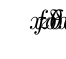
\begin{tikzpicture}
    \node (in)
        [inner sep=0]
        {\tikz \drawMessagesWithArrows{$x$}{\ $\delta x$}{\ $\average{\HeCal x}$\ }{\hNodeDistance};};
    \node (module)
         [anchor=south west, inner sep=0]
         at (in.south east)
         {\tikz \drawModuleWithParams{$f$}{16}{$\theta$}{\ $\average{\delta\theta}$\ }{\ $\average{\HeCal \theta}$\ };};
    \node (out)
        [inner sep=0, anchor=south west]
        at (module.south east)
         {\tikz \drawMessagesWithArrows{$z$}{$\delta z$}{\ $\average{\HeCal z}$\ }{\hNodeDistance};};	
\end{tikzpicture}